\documentclass[10pt,a4paper]{article}

\usepackage[utf8]{inputenc}
\usepackage[T1]{fontenc}
\usepackage{lmodern}
\usepackage[english]{babel}
\usepackage{amsmath,amssymb}
\usepackage{geometry}
\usepackage{hyperref}
\usepackage{enumitem}
\usepackage{tikz}
\usetikzlibrary{arrows.meta, positioning}
\usepackage{graphicx}
\usepackage{algorithm}
\usepackage{algpseudocode}
\geometry{margin=2.2cm}

\title{\vspace{-1.5em}Adaptive Software Visualization:\\
\large a position paper on a formal model of the text/diagram ratio with AI delegation}
\author{Kristian Sestak}
\date{}

\begin{document}
\maketitle
\vspace{-2em}

\begin{abstract}
\noindent
This is a \textbf{position paper}: we propose a formal framework for the
design of learning materials in software engineering that explicitly
separates \emph{data transmission} (Shannon channel) from the
\emph{reconstruction} of information, knowledge and wisdom on the
receiver's side (DIKW). A material is parametrized by the vector
$(p, J, \sigma, \eta)$ – the diagram-to-text area ratio, linguistic
simplicity, spatial integration, and the degree of detail delegation to
an LLM. We define a utility function $E$ and present two main findings:
(i) $E$ decomposes into three independently regulable components –
\emph{transmission}, \emph{reconstruction loss} and \emph{load};
(ii) the optimal ratio $p^{*} \in [1.5, 2.0]$ is a \emph{prediction
derived} from Cowan's working memory model and Paivio's dual coding
theory, not a postulate. We formulate five testable hypotheses and
illustrate the framework on the \emph{Observer} design pattern.
Empirical validation is the subject of a planned pilot; the goal of
this work is a \textbf{research agenda} and a conceptual contribution.

\smallskip
\noindent\textbf{Keywords:} software visualization, cognitive load,
DIKW, LLM-assisted learning, multimedia learning, contextual bandit,
Shannon channel.
\end{abstract}

\section{Introduction and Contributions}

\paragraph{Motivation.}
The complexity of modern software systems grows orders of magnitude
faster than the capacity of the human cognitive apparatus: millions of
lines of code, hundreds of microservices, heterogeneous APIs and data
flows. Effective extraction of information and knowledge from this
volume of data hits \emph{two hard limits}. (i) The \textbf{transmission
channel} (screen, printed page, attention) has a finite Shannon capacity
$C_{\text{ch}}$, so arbitrarily dense content cannot be transmitted
without loss. (ii) The \textbf{human brain} has an empirically bounded
working memory capacity ($C_{\text{wm}} \approx 4$ chunks
\cite{cowan2001}) and a bounded sequential reading rate
($\sim\!250$ words/min). These bounds are fixed; they do not scale with
system complexity. The key question therefore is not \emph{how much}
information we transmit, but \emph{how to combine it effectively}:
what type of text (sentence length, technical density), what type of
diagrams (UML, flow graphs, sequence), how many nodes and edges for a
given task, how to annotate, and when to delegate details to AI.
Without a formal criterion this choice remains intuitive.

The design of learning materials balances between text and diagrams
without an established quantitative criterion. The rise of LLMs
transforms this problem in two ways: (i) details (syntax, API) can be
delegated to AI, and (ii) content can be generated adaptively. Yet a
\emph{formal framework} connecting these possibilities with cognitive
load theory \cite{sweller2019} and multimedia learning \cite{mayer2021}
is missing.

\paragraph{Contributions (C1--C4).}
\textbf{C1} – a channel-reconstruction decomposition separates the
Shannon transmission of $d$ from DIKW reconstruction
$\iota, \kappa, \omega$.
\textbf{C2} – a unified model with parameters $(p, J, \sigma, \eta)$
and a utility function $E$.
\textbf{C3} – formulation of an adaptive policy as a contextual bandit.
\textbf{C4} – five testable hypotheses $H_1$--$H_5$ with an effect
threshold and a pilot experiment plan.

\paragraph{Paper structure.} Section~2 summarizes related work.
Section~3 introduces the channel/DIKW separation. Section~4 defines
the parameters $(p, J, \sigma, \eta)$. Section~5 formulates the
optimization problem. Section~6 demonstrates the framework on the
\emph{Observer} pattern. Section~7 grounds the parameters in the
literature. Section~8 formulates the hypotheses; Section~9 contains
the conclusion and recommendations.

\section{Related Work}

The framework builds on \emph{cognitive load theory}
\cite{sweller1988,sweller2019} (intrinsic, extraneous, germane load),
\emph{multimedia learning theory} \cite{mayer2021} (principles of
\emph{modality}, \emph{spatial contiguity} – represented in our model
by $\sigma$), and on surveys of \emph{software visualization}
\cite{teyseyre2009,merino2018}. Van Wijk's value-of-visualization model
\cite{vanwijk2005} motivates the utility function $E$; Shannon's theory
\cite{shannon1948} and the DIKW hierarchy \cite{ackoff1989,rowley2007}
motivate the separation of transmission from reconstruction. On the
learner-model side we use \emph{Bayesian Knowledge Tracing}
\cite{corbett1995}, contextual bandits \cite{li2010}, and NASA-TLX
\cite{hart1988}. Compared to existing literature we integrate AI
delegation via $\eta$ and explicitly separate channel and semantic
entropy.

\section{Information Channel vs.\ DIKW}

\textbf{Claim.} Only \emph{data} pass through the communication channel;
information, knowledge and wisdom emerge only through reconstruction on
the receiver's side.

Let $d$ be the data signal and $S$ the receiver's state (prior
knowledge, goals $G$). Then
\begin{equation}
I = \iota(d, S),\quad K = \kappa(I, S),\quad W = \omega(K, S, G).
\end{equation}

\begin{figure}[h]
\centering
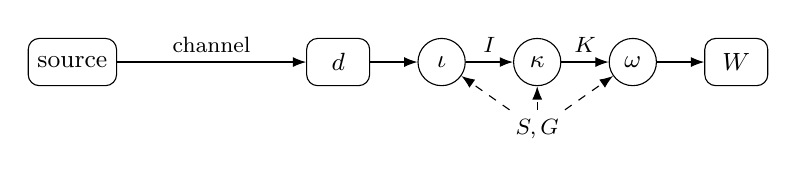
\begin{tikzpicture}[
  node distance=7mm and 6mm,
  box/.style={draw, rounded corners, minimum height=6mm, minimum width=8mm, align=center, font=\small},
  op/.style={draw, circle, minimum size=6mm, inner sep=0pt, font=\small},
  >=Latex
]
  \node[box] (src) {source};
  \node[box, right=24mm of src] (d) {$d$};
  \node[op, right=of d] (iota) {$\iota$};
  \node[op, right=of iota] (kappa) {$\kappa$};
  \node[op, right=of kappa] (omega) {$\omega$};
  \node[box, right=of omega] (rec) {$W$};
  \node[below=3mm of kappa, font=\footnotesize] (S) {$S, G$};
  \draw[->] (src) -- node[above, font=\footnotesize]{channel} (d);
  \draw[->] (d) -- (iota);
  \draw[->] (iota) -- node[above, font=\footnotesize]{$I$} (kappa);
  \draw[->] (kappa) -- node[above, font=\footnotesize]{$K$} (omega);
  \draw[->] (omega) -- (rec);
  \draw[dashed, ->] (S) -- (iota);
  \draw[dashed, ->] (S) -- (kappa);
  \draw[dashed, ->] (S) -- (omega);
\end{tikzpicture}
\caption{Only data $d$ pass through the channel; $I, K, W$ emerge via
reconstruction conditioned on state $S$ and goals $G$.}
\label{fig:channel}
\end{figure}

\paragraph{Channel and semantic entropy.}
The channel has capacity $C_{\text{ch}} = \max_{P(x)} I(X;Y)$ and a
residual loss $H(X\mid Y) = H(X) - I(X;Y)$. On the receiver's side an
additional \emph{semantic entropy} arises:
\begin{equation}
H_{\iota}(I \mid d, S) = -\sum_{I} P(I\mid d, S)\log P(I\mid d, S),
\end{equation}
which quantifies the ambiguity of interpretation. Material design must
minimize both sources of loss.

\section{Material Parametrization}

\begin{table}[h]
\centering
\small
\caption{Notation.}
\label{tab:notation}
\begin{tabular}{ll}
\hline
Symbol & Meaning \\
\hline
$d$ & data signal transmitted by the channel \\
$S, G$ & receiver state, receiver's goals \\
$\iota, \kappa, \omega$ & data $\to I$, $I \to K$, $K \to W$ \\
$I, K, W$ & information, knowledge, wisdom \\
$H(X\mid Y)$ & channel entropy \\
$H_{\iota}$ & semantic entropy of reconstruction \\
$C_{\text{ch}}$ & Shannon channel capacity \\
$C_{\text{wm}}$ & working memory capacity \\
$p$ & diagram/text area ratio \\
$J$ & linguistic simplicity \\
$\sigma$ & text--diagram spatial integration \\
$\eta$ & degree of detail delegation to AI \\
$L_{\text{tot}}$ & total cognitive load (CLT) \\
$\lambda$ & learning rate (Van Wijk) \\
$E$ & material utility function \\
$\theta_t$ & learner knowledge state (BKT) \\
\hline
\end{tabular}
\end{table}

\paragraph{$p$ – diagram/text ratio.}
$p = A_d / A_t$, where $A_d, A_t$ are the areas of diagrams and text at
a fixed DPI.

\paragraph{$J$ – linguistic simplicity.}
$J(T) = \frac{1}{|T|}\sum_{w \in T} \varphi(\log f_C(w))$ with
$\varphi = 1 - \log\mathrm{rank}_C(w)/\log|V_C|$; corpus:
SUBTLEX for English, equivalent frequency corpus for other languages.

\paragraph{$\sigma$ – spatial integration.}
$\sigma \in [0,1]$: $1$ = fully annotated diagram (text placed next to
elements), $0$ = separated panels. Operationalizes the principle of
\emph{spatial contiguity} \cite{mayer2021}.

\paragraph{$\eta$ – AI delegation level.}
$\eta \in [0,1]$: $K_{\text{actual}} = K_A + \eta\, K_{D \to \text{AI}}$,
where $A$ are abstractions (non-transferable) and $D$ are details
(delegable).

\section{Formal Problem}

Cognitive load following CLT:
\begin{equation}
L_{\text{tot}} = L_{\text{int}} + \alpha(1-J) + \beta g(p) + \gamma(1-\sigma),
\end{equation}
where $g$ has a U-shape with a minimum at $p^{*}$. Learning curve
(Van Wijk): $K(t) = K_{\max}(1 - e^{-\lambda t})$ with
$\lambda = \lambda_0 J \sigma h(p)$. Utility function:
\begin{equation}
E = \int_0^T \dot K(t)\bigl(1 - L_{\text{tot}}(t)\bigr)\,dt.
\end{equation}
Decomposition:
\begin{equation}
E = \underbrace{\int I(X;Y)\,dt}_{\text{transmission}}
  - \underbrace{\int H_{\iota}(I\mid d,S)\,dt}_{\text{reconstruction}}
  - \mu\!\int L_{\text{tot}}(t)\,dt.
\end{equation}

\begin{figure}[h]
\centering
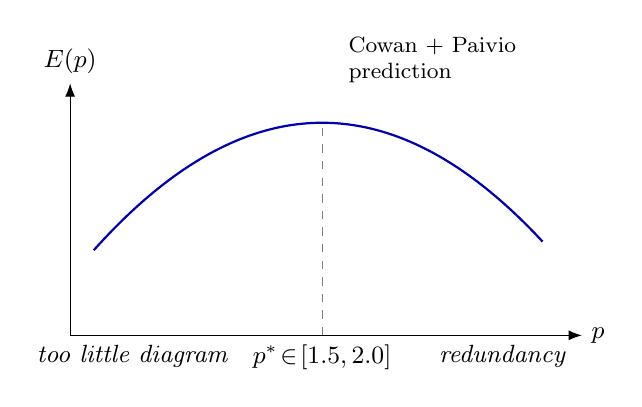
\begin{tikzpicture}[>=Latex]
  \draw[->] (0,0) -- (6.5,0) node[right, font=\small]{$p$};
  \draw[->] (0,0) -- (0,3.2) node[above, font=\small]{$E(p)$};
  \draw[thick, blue!70!black, domain=0.3:6, smooth, samples=60]
      plot (\x, {2.7 - 0.55*(\x-3.2)*(\x-3.2)*0.35});
  \draw[dashed, gray] (3.2,0) -- (3.2,2.7);
  \node[below, font=\small] at (3.2,0) {$p^{*}\!\in\![1.5,2.0]$};
  \node[below, font=\small] at (0.8,0) {\emph{too little diagram}};
  \node[below, font=\small] at (5.5,0) {\emph{redundancy}};
  \node[font=\footnotesize, align=left] at (4.6,3.5) {Cowan + Paivio\\prediction};
\end{tikzpicture}
\caption{Schematic shape of the utility function $E(p)$ at fixed
$J, \sigma, \eta$. The optimum $p^{*} \in [1.5, 2.0]$ is a prediction
from working memory capacity \cite{cowan2001} and dual coding
\cite{paivio1990}.}
\label{fig:epcurve}
\end{figure}

We seek a policy $\pi^{*}: S_t \to (p, J, \sigma, \eta)$ that
maximizes $\mathbb{E}[E]$ subject to $C_{\text{ch}} \geq R(d_t)$,
$L_{\text{tot}} \leq L_{\max}$, $H_{\iota} \leq \varepsilon_{\iota}$,
$\eta \leq \eta_{\max}(S_t)$.

\paragraph{Solution.} We solve the problem via \emph{online adaptation},
the methodologically preferred approach for tasks with unknown reward
functions and heterogeneous users: we formulate it as a contextual
bandit \cite{li2010} over the state $S_t = (\theta_t, L_t, \eta_t)$,
with $\theta_t$ updated via BKT \cite{corbett1995} and $L_t$ via an
exponential filter over sensors (error rate, time on page, NASA-TLX
\cite{hart1988}). The coefficients $\alpha, \beta, \gamma, \lambda_0$
are estimated jointly with the policy optimization.

\begin{algorithm}[h]
\small
\caption{Adaptive policy $\pi$ (contextual bandit)}
\label{alg:policy}
\begin{algorithmic}[1]
  \State \textbf{input:} priors $\theta_0$, $L_0$; horizon $T$; discount $\mu$
  \For{$t = 1, \dots, T$}
    \State $S_t \gets (\theta_{t-1}, L_{t-1}, \eta_{t-1})$
    \State $(p, J, \sigma, \eta) \gets \pi_\phi(S_t)$ \Comment{Thompson sampling}
    \State $d_t \gets \textsc{LLM.generate}(\text{concept}, p, J, \sigma, \eta)$
    \State present $d_t$ to the learner; collect sensors
    \State $r_t \gets \Delta \theta_t - \mu\, \hat L_t$
    \State update $\theta_t$ (BKT), $L_t$ (filter), parameters $\phi$
  \EndFor
\end{algorithmic}
\end{algorithm}

\section{Worked Example: Observer Pattern}

To illustrate the parametrization we compare three versions of the
material for the \emph{Observer} design pattern:

\begin{center}
\small
\begin{tabular}{lcccc}
\hline
Version & $p$ & $J$ & $\sigma$ & $\eta$ \\
\hline
V\textsubscript{A} textbook (GoF) & 0.25 & 0.42 & 0.20 & 0.0 \\
V\textsubscript{B} annotated UML  & 1.40 & 0.68 & 0.85 & 0.0 \\
V\textsubscript{C} + AI assistant & 1.40 & 0.68 & 0.85 & 0.6 \\
\hline
\end{tabular}
\end{center}

V\textsubscript{A} represents the classical textbook approach (long
text, small separated UML). V\textsubscript{B} shifts the ratio towards
the diagram and places annotations directly at the
\texttt{Subject}/\texttt{Observer} classes. V\textsubscript{C}
additionally adds an AI assistant for syntactic details.

\begin{figure}[h]
\centering
\begin{minipage}[b]{0.47\linewidth}
  \centering
  \includegraphics[width=\linewidth]{obrazky/V_A.png}
  \small (a) V\textsubscript{A}: bare UML, $\sigma \approx 0.2$.
\end{minipage}\hfill
\begin{minipage}[b]{0.47\linewidth}
  \centering
  \includegraphics[width=\linewidth]{obrazky/V_B.png}
  \small (b) V\textsubscript{B}: annotated UML, $\sigma \approx 0.85$.
\end{minipage}
\caption{Contrast between the separated (V\textsubscript{A}) and the
spatially integrated (V\textsubscript{B}) representation of the
\emph{Observer} pattern. Annotations placed directly at elements
eliminate the split-attention effect.}
\label{fig:observer}
\end{figure}

\paragraph{Content split in V\textsubscript{C}.}
Concrete distribution among diagram, text and delegated details:

\begin{center}
\small
\begin{tabular}{p{0.28\linewidth} p{0.30\linewidth} p{0.32\linewidth}}
\hline
\textbf{Diagram ($A_d$, $\sigma{=}0.85$)} &
\textbf{Text ($A_t$, $J{=}0.68$)} &
\textbf{AI ($\eta{=}0.6$)} \\
\hline
UML: \texttt{Subject}, \texttt{Observer}, \texttt{*} association,
annotated arrows \texttt{notify()}, \texttt{update()} &
\emph{Abstraction} ($K_A$): publisher/subscriber separation,
rationale (loose coupling), when to use, when not to &
\emph{Details} ($K_D$): Java \texttt{Observable}, Python
\texttt{weakref}, concurrency pitfalls, gotchas \\
\hline
\end{tabular}
\end{center}

The abstractions $K_A$ (which the human \emph{must} know) reside in
text and diagram; the details $K_D$ are delegated to AI so that they
do not burden working memory while the mental model is being built.
Model prediction: at equal $T$, $E(V_C) > E(V_B) > E(V_A)$, since
$\lambda \propto J\sigma$ grows (V\textsubscript{A}$\to$V\textsubscript{B})
and $L_{\text{int}}$ decreases with $\eta$
(V\textsubscript{B}$\to$V\textsubscript{C}). Empirical verification
is part of the upcoming pilot.

\section{Theoretical Grounding of the Parameters}

The parameters $(p, J, \sigma, \eta)$ are not freely chosen; each has
a \emph{first-principle bound} and an \emph{empirical anchor} in the
literature. Empirical validation calibrates coefficients, not structure.

\paragraph{$\sigma$ – strongest support.}
The \emph{spatial contiguity} principle \cite{mayer2021} is confirmed
by a meta-analysis \cite{ginns2006} with effect size $d \approx 0.85$.
Prediction: $\sigma \to 1$ improves learning by $\sim 0.8$\,SD over
separated panels. \emph{Default:} $\sigma = 0.85$.

\paragraph{$J$ – psycholinguistically anchored.}
Zipf's law gives $\log f_C(w) \approx \log N - \log \mathrm{rank}_C(w)$,
which directly motivates the form of $\varphi$. Lexical decision tasks
\cite{brysbaert2018} show a reaction-time decrease of $\sim\!30$\,ms
per log-frequency unit; convergent validation is provided by
readability metrics (Flesch-Kincaid, SMOG). \emph{Default:} target
$J \in [0.6, 0.8]$ for adult learners.

\paragraph{$p$ – derived from working memory.}
By Cowan's model \cite{cowan2001} working memory capacity is
$C_{\text{wm}} \approx 4 \pm 1$ chunks. By dual coding theory
\cite{paivio1990} a diagram encodes $r$ relational chunks in parallel,
while text encodes $s$ sequential steps in time $\tau_{\text{verb}}$.
$L_{\text{ext}}$ is minimized at channel balance:
\begin{equation}
p^{*} \approx \frac{r}{s}\cdot \frac{\tau_{\text{vis}}}{\tau_{\text{verb}}}.
\end{equation}
For typical software concepts (class/sequence diagrams:
$r/s \in [1.5, 2]$) and $\tau_{\text{vis}}/\tau_{\text{verb}} \approx 1$
we obtain $p^{*} \in [1.5, 2.0]$. \emph{This interval is not a postulate
but a prediction from Cowan and Paivio}; empirical calibration will
refine the ratio $\tau_{\text{vis}}/\tau_{\text{verb}}$.

\paragraph{$\eta$ – conditioned on expertise.}
\emph{Cognitive offloading} \cite{riskogilbert2016} shows that rational
delegation grows with intrinsic load. The \emph{expertise reversal
effect} \cite{kalyuga2007} implies that for novices $\eta^{*}$ is high,
while for experts it is low (otherwise they will not learn the details
$K_D$). We propose
\begin{equation}
\eta^{*}(S) = \eta_0 \bigl(1 - \theta_{\text{prior}}(S)\bigr),
\end{equation}
where $\theta_{\text{prior}} \in [0,1]$ is the average prior knowledge
of details in state $S$. \emph{Default:} $\eta_0 = 0.7$ for novices,
decreasing as $\theta$ grows.

\medskip
\noindent \textbf{Summary.} Three of the four parameters
($\sigma, J, p$) have either a direct meta-analytic anchor or a
derivation from established working-memory capacity limits; $\eta$ is
the most weakly supported theoretically and is therefore the primary
target of empirical validation.

\section{Hypotheses and Pilot Plan}

\textbf{Baseline:} V\textsubscript{A} (textbook material,
$p\!\approx\!0.3$).
\textbf{Primary metric:} transfer score after 7 days.
\textbf{Threshold:} $\geq 5$ p.p., Cohen's $d \geq 0.3$,
$n \geq 64$ per group.

\begin{description}[leftmargin=2em, style=nextline, itemsep=0pt]
  \item[$H_1$] Higher $J$ improves $P(\hat K = K^{*})$ by $\geq 5$ p.p.
  \item[$H_2$] $p^{*} \in [1.5, 2.0]$ maximizes $E$ for adult learners.
  \item[$H_3$] Higher $\sigma$ lowers NASA-TLX at fixed $p$.
  \item[$H_4$] Delegation ($\eta > 0$) increases $K_A$, not $K_D$.
  \item[$H_5$] The adaptive policy outperforms the static baseline on retention.
\end{description}

\paragraph{Falsification criteria.}
To preserve scientific credibility we fix in advance the conditions
under which we \emph{reject} the framework's predictions:
(F1) if the pilot shows $p^{*} < 0.8$ or $p^{*} > 2.5$, the Cowan+Paivio
prediction is falsified and the derivation of $p^{*}$ requires revision;
(F2) if the effect of $\sigma$ on the transfer score is $d < 0.2$, the
spatial contiguity anchor from \cite{ginns2006} did not replicate in
our context;
(F3) if $\eta > 0$ does not improve $K_A$ nor reduce $L_{\text{int}}$,
the assumption of detail delegation does not hold and the model must
be reformulated.

\paragraph{Framework limits.}
The framework \emph{does not address} three areas that are deliberately
out of scope:
(i) the \emph{affective component} of learning (motivation, frustration,
engagement), modeled e.g.\ by self-determination theory;
(ii) \emph{collaborative learning} – the framework assumes an
individual learner, not a dyad or group;
(iii) \emph{long-term retention} beyond $\sim\!30$ days, where
spaced-repetition mechanisms dominate and would require an orthogonal
extension. The framework also \emph{assumes reliability of the AI
assistant}; hallucinations of $K_D$ break the identity
$K_{\text{actual}} = K_A + \eta K_D$ and effectively lower $\eta^{*}$ –
quantifying this effect belongs to an extension.

\paragraph{Threats to validity.} Construct: $J$ ignores syntactic depth
and discourse coherence. Internal: novelty-vs.-adaptivity confound in
$H_5$. External: single-cohort sample. Ethics: sensors require informed
consent and GDPR-compliant processing.

\section{Conclusion}

\paragraph{Contribution summary.}
We proposed a position-paper framework responding to the growing
complexity of software systems under fixed limits of channel capacity
$C_{\text{ch}}$ and working memory $C_{\text{wm}} \approx 4$
\cite{cowan2001}. The framework (i) separates the Shannon transmission
of $d$ from DIKW reconstruction via the operators $\iota, \kappa,
\omega$, (ii) distinguishes \emph{channel entropy} $H(X\mid Y)$ from
\emph{semantic entropy} $H_{\iota}(I\mid d, S)$ as two independent
sources of loss, (iii) operationalizes the four design parameters
$(p, J, \sigma, \eta)$, and (iv) formulates the optimization of the
utility function $E$ as an online contextual bandit.

\paragraph{New findings of this contribution.}
The parameters are not freely chosen: $\sigma$ has a meta-analytic
anchor $d \approx 0.85$ \cite{ginns2006}, $J$ a psycholinguistic one
\cite{brysbaert2018}, and $p^{*} \in [1.5, 2.0]$ is a
\emph{prediction derived} from Cowan and Paivio
\cite{cowan2001,paivio1990}, not a postulate. The delegation $\eta^{*}$
is conditioned on expertise by the \emph{expertise reversal effect}
\cite{kalyuga2007}. The decomposition
$E = \text{transmission} - \text{reconstruction loss} - \text{load}$
identifies three independently regulable components of material design.

\paragraph{Practical recommendations.}
(a) \textbf{Measure, don't guess:} quantify $(p, J, \sigma)$ for each
material before publishing; default targets $p \in [1.5, 2.0]$,
$J \in [0.6, 0.8]$, $\sigma \geq 0.8$.
(b) \textbf{Prefer annotated diagrams} over separated panels (strong
$\sigma$ anchor).
(c) \textbf{Scale $\eta$ with expertise:} $\eta \approx 0.7$ for
novices, $\eta \to 0$ for experts to prevent atrophy of $K_D$.
(d) \textbf{Bound diagram complexity} relative to $C_{\text{wm}}$:
split or hierarchize graphs with more than $7$--$9$ nodes per screen.
(e) \textbf{Test transfer ($K_A$) and recall ($K_D$) separately} so
that AI delegation does not confound the measured knowledge.

\paragraph{Next steps.}
A pilot experiment ($n \geq 64$ per group) calibrating the coefficients
$\alpha, \beta, \gamma, \lambda_0$ and testing $H_1$--$H_5$. Extension
of $J$ by syntactic depth and discourse coherence. Exploration of
domains beyond software engineering (mathematics, medicine) for
external validity. In the long run the framework points towards a
conversational interface in which text and diagrams are merely
transient artifacts of the reconstruction of $I, K, W$ in the human
mind; machines remain in the domain of $d$, the human remains in the
domain of $\omega$ (goal evaluation).

\begin{thebibliography}{99}
\small
\bibitem{shannon1948} C.~E. Shannon, ``A mathematical theory of communication,'' \emph{Bell Syst.\ Tech.\ J.}, vol.~27, pp.~379--423, 1948.
\bibitem{ackoff1989} R.~L. Ackoff, ``From data to wisdom,'' \emph{J.\ Appl.\ Syst.\ Anal.}, vol.~16, pp.~3--9, 1989.
\bibitem{rowley2007} J.~Rowley, ``The wisdom hierarchy: representations of the DIKW hierarchy,'' \emph{J.\ Inf.\ Sci.}, vol.~33, no.~2, pp.~163--180, 2007.
\bibitem{sweller1988} J.~Sweller, ``Cognitive load during problem solving,'' \emph{Cogn.\ Sci.}, vol.~12, pp.~257--285, 1988.
\bibitem{sweller2019} J.~Sweller, J.~J.~G. van~Merriënboer, F.~Paas, ``Cognitive architecture and instructional design: 20 year update,'' \emph{Educ.\ Psychol.\ Rev.}, vol.~31, pp.~261--292, 2019.
\bibitem{mayer2021} R.~E. Mayer, \emph{Multimedia Learning}, 3rd ed., Cambridge Univ.\ Press, 2021.
\bibitem{vanwijk2005} J.~J. van~Wijk, ``The value of visualization,'' \emph{IEEE Visualization}, 2005, pp.~79--86.
\bibitem{teyseyre2009} A.~R. Teyseyre, M.~R. Campo, ``An overview of 3D software visualization,'' \emph{IEEE TVCG}, vol.~15, no.~1, pp.~87--105, 2009.
\bibitem{merino2018} L.~Merino et al., ``A systematic literature review of software visualization evaluation,'' \emph{JSS}, vol.~144, pp.~165--180, 2018.
\bibitem{corbett1995} A.~T. Corbett, J.~R. Anderson, ``Knowledge tracing,'' \emph{UMUAI}, vol.~4, pp.~253--278, 1995.
\bibitem{li2010} L.~Li et al., ``A contextual-bandit approach to personalized news article recommendation,'' \emph{WWW}, 2010, pp.~661--670.
\bibitem{hart1988} S.~G. Hart, L.~E. Staveland, ``Development of NASA-TLX,'' \emph{Adv.\ Psychol.}, vol.~52, pp.~139--183, 1988.
\bibitem{ginns2006} P.~Ginns, ``Integrating information: A meta-analysis of the spatial contiguity and temporal contiguity effects,'' \emph{Learning and Instruction}, vol.~16, no.~6, pp.~511--525, 2006.
\bibitem{brysbaert2018} M.~Brysbaert, P.~Mandera, E.~Keuleers, ``The word frequency effect in word processing: An updated review,'' \emph{Current Directions in Psychological Science}, vol.~27, no.~1, pp.~45--50, 2018.
\bibitem{cowan2001} N.~Cowan, ``The magical number 4 in short-term memory: A reconsideration of mental storage capacity,'' \emph{Behavioral and Brain Sciences}, vol.~24, no.~1, pp.~87--114, 2001.
\bibitem{paivio1990} A.~Paivio, \emph{Mental Representations: A Dual Coding Approach}, Oxford Univ.\ Press, 1990.
\bibitem{riskogilbert2016} E.~F. Risko, S.~J. Gilbert, ``Cognitive offloading,'' \emph{Trends in Cognitive Sciences}, vol.~20, no.~9, pp.~676--688, 2016.
\bibitem{kalyuga2007} S.~Kalyuga, ``Expertise reversal effect and its implications for learner-tailored instruction,'' \emph{Educational Psychology Review}, vol.~19, pp.~509--539, 2007.
\end{thebibliography}

\end{document}
